%\chapter{Analysis and Design}
\chapter{Analiză și proiectare}
\label{cap:analiza-si-proiectare}

In acest capitol este descris design-ul proiectului si cuprinde: cerintele sistemului, specificatiile cazurilor de utilizare, arhitectura sistemului, comportamentul sistemului, datele utilizate de sistem, dependintele sistemului si algoritmi esentiali si metodele folosite. Descrierea acestora se realizeaza prin asocierea cu diagramelor aferente.

\section{Cerintele sistemului}

Sistemul propus \textit{\thesistitle} reprezinta un software gratis care ofera clientului atat caracteristici specificie unui reverse proxy, cat si modalitati de protectie asemeni unui sistem de prevenire a intruziunilor.
Sistemul este usor de instalat si de utilizat, chiar si de catre utilizatorii neexperimentati, oferindu-le acestora o interfata clara si sugestiva, ce mascheaza logica complicata din spate. In spate, sistemul ofera un reverse proxy ce intercepteaza tot traficul destinat catre un anumit server, de pe una sau mai multe interfete. In procesul de interceptare, acesta implementeaza si cateva modalitati de prevenire a unor tentative de intruziune. Sistemul blocheaza toate ip-urile utilizate frecevent de reteaua Tor in ultima luna si atacurile de SQL injection cu o acuratete de 90\%.

Sistemul trebui sa indeplineasca urmatoarele cerinte \textbf{functionale}:
\begin{enumerate}
	\item Sa realizere conexiunea la un server HTTP/HTTPS si sa redirectioneze traficul primit catre acesta.
	\item Sa intercepteze traficul venit pe o anumita interfata si port prestabilit.
	\item Sa prelucreze request-urile primite de la clineti intr-un format specific clasificatorului de SQL injection.
	\item Sa nu redirectioneze reqesturile clasificate ca si SQL injection.
	\item Sa blocheze conectarea clientilor ce folosesc ip-uri clasificate ca ip-uri de Tor.
	\item Sa permita utilizatorului sa editez si sa vizualizeze lista ip-urilor de Tor.
	\item Sa prezinte in interfata grafica toate interventiile rezlizate asupra traficului(blocari de conexiuni sau de request-uri).
	\item Sa permita utilizatorului sa configureze modul de operare al sistemului.
\end{enumerate}

Sistemul trebuie, de asemenea, să aibă următoarele caracteristici \textbf{non-funcționale}:
\begin{enumerate}
	\item Sa fie usor de instalat si de folosit pentru orice utilizator, oricat de neexperimentat.
	\item Sa poata intercepta traficul de pe orice/oricate interfete disponibile.
	\item Sa poata rula pe orice sistem de operare Windows cu Python2 instalat.
	\item Sa aiba o rata de blocare de 100\% a ip-urilor de pe lista neagra, iar
	in cazul detectiei de SQL injection sa nu aiba detectii false pozitive mai mari 2-3\%
	si o acuratete generala de peste 90\%
\end{enumerate}
\newpage

\section{Specificatiile cazurilor de utilizare}

\subsection{Actori, stakeholders si interese}

Principalii actori si stakeholder-i sunt administratorii de servere, respectiv de baze de date. In implementarea sistemului propus se urmareste satisfacerea nevoilor acestor persoane, oferindule un plus de securitate asupra datelor ce sunt accesate de catre clienti, respectiv impotriva clientilor rau intentionati. Interesele acestor comunitati de utilizatori sunt urmarite pentru a livra un produs care sa ofere aceste protectii intr-o maniera cat de prietenoasa pentru utilizator si cat mai eficienta.

\subsection{Basic flow}

\begin{figure}[h]
	\centering
	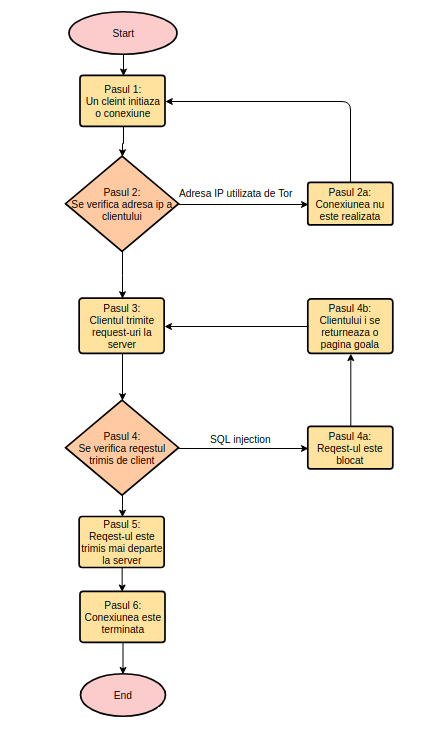
\includegraphics[width=0.4\textwidth]{basicflow.png}
	\caption{Basic flow pentru evenimente}
	\label{fig:basic-flow}
\end{figure}
Figura ~\ref{fig:basic-flow} prezinta cum arata basic flow-ul pentru evenimentele din sistemul propus. \\

Evenimentele sistemului:
\begin{enumerate}
	\item \textbf{Start}: aceste cazuri de utilizare sunt initiate in momentul in care sistemul este plasat intre un server si utilizatorii acestuia.
	\item \textbf{Pasul 1}: un client doreste si initializeze o conexiune la server.
	\item \textbf{Pasul 2}: adresa ip a clientului este verificata ca acesta sa nu fie un utilizator de Tor.
	\item \textbf{Pasul 3}: clientul comunica cu serverul prin reqest-uri individuale.
	\item \textbf{Pasul 4}: reqest-urile sunt verificate ca acestea sa nu fie atacuri de SQL injection.
	\item \textbf{Pasul 5}: request-urile sunt trimise mai departe catre server.
	\item \textbf{Pasul 6}: conexiunea este terminata(de catre client sau server).
	\item \textbf{End}: la sfarsitul unui sir de evenimente, utilizatorul sistemului poate sa vada daca clientul ce a initializat evenimentele a realizat actiuni considerate ca malitioase.
	
	
\end{enumerate}


\subsection{Alternative flow}
Evenimentele alternative in cazurile de utilizare sunt urmatoarele:
\begin{enumerate}
	\item \textbf{Pasul 2a}: in cazul in care un utilizator cu adresa ip de Tor incearca sa realizeze conexiunea la server aceasta este refuzata. 
	\item \textbf{Pasul 4a}: in cazul in care un utilizator incearca sa trimita la server un request ce reprezinta o tentativa de atac SQL injection, acesta este blocat.
	\item \textbf{Pasul 4b}: pentru request-urile blocate ca si SQL injection clientului i se returneaza o pagina goala. 
\end{enumerate}

\newpage


\section{Arhitectura sistemului si modulele principale}

In conformitate cu cerintele sistemului si specificatiile cazurilor de utilizare, sistemul propus este alcatuit din module specifice care sa trateze in mod individual problemele majore ridicate de sistem, printr-o implementare modulara, oferind astfel usurinta implementarii de noi functionalitati.

\begin{figure}[h]
	\centering
	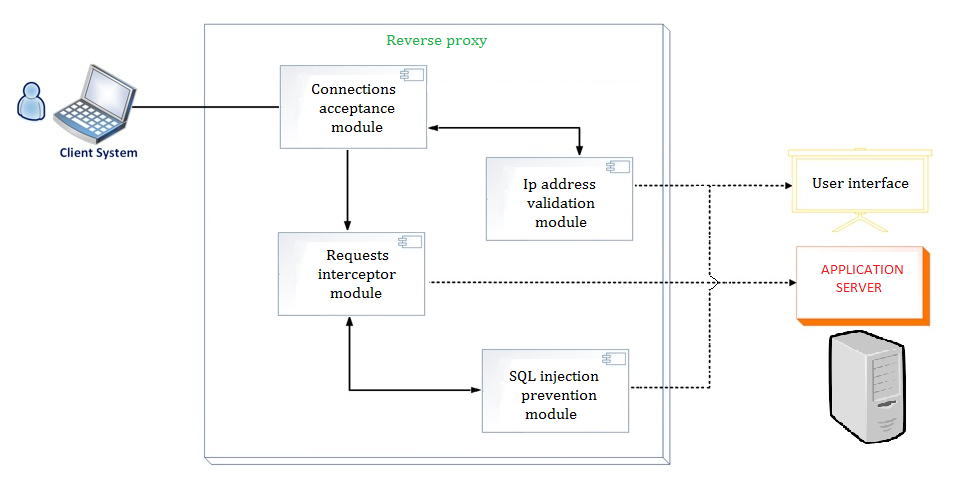
\includegraphics[width=0.8\textwidth]{module.png}
	\caption{Principalele module ale sitemului propus}
	\label{fig:module}
\end{figure}
Figura ~\ref{fig:module} prezinta care sunt pricipalele module ale sistemului propus, precum si interactiunea dintre acestea. \\

Principala si teoretic singura componenta a sistemului este reprezentata de cea de \textbf{reverse proxy}, insa petru a obtine rezultatele dorite si pentru a incorpora functionalitatile de protecti in aceasta, logica ei a fost impartita in cele 4 mari submodule:\textbf{connections acceptance module} si \textbf{request interceptor module}, ce reprezinta componentele ce suporta logica unui reverse proxy si \textbf{ip address validation module} si \textbf{SQL injection prevention module}, ce reprezinta modulele care interactioneaza cu cele ce implementeaza structura de reverse proxy pentru a oferi functionalitatile de securitate.\\




\textbf{Client system} si  \textbf{application server}.\\ 

Aceste doua componente reprezinta componetele clasice intre care vin plasat sistemul propus. \textbf{Client system} este reprezentat de orice client doreste sa acceseze baza de date/parte de server a unei aplicatii. \textbf{Application server} reprezinta serverul aplicatie la care se pot conecta clientii pentru a avea acces la un anumit continut. Sistemul propus are rolul de intermediere intre cele doua tipuri de componente, prevenind astfel eventuale tentative de expluatare a unor vulnerabilitati din partea clientului catre server.


\textbf{Connections acceptance module}.\\

Acest modul este constituit din componentele oferite de biblioteca open source \textbf{twisted}, fiind modificate ulterior pentru a permite integrarea modulului \textbf{Ip address validation module} . Modulul are rolul de a crea un socket pe sistemul pe care ruleaza acesta, care sa asculte pentru posibile conexiunui. In cazul in care un client incearca sa initieze o noua conexiune acesta trasmite adresa ip a clietului catre modului \textbf{Ip address validation module}, iar in functie de raspunsul acestuia conexiunea acestuia va fi realizata sau refuzata.\\ 


 \textbf{Request interceptor module}.\\
 
 Asemeni modulului anterior, \textbf{Connections acceptance module}, acest modul este construit peste codul oferit de biblioteca open source \textbf{twisted}. Biblioteca ofera suport pentru interceptarea reqest-urilor dintre un client si server, implementandu-se o logica suplimentarea ce incorporeaza modulul de detectie a atacurilor SQLI( \textbf{SQL injection prevention module}). In acest modul se interpreteaza natura URL-urilor trimise de catre client catre server.
 Interpretarea constand in analiza URI-ului unui request de catre modulul de prevenire a atacurilor SQLI, iar in functie de rezultatul acestuia returnand raspunsuri corespunzatoare atat clientului cat si serverului(in caz de tentatica de atac, la server nu ca ajunge nimic). \\
 
\textbf{Ip address validation module}. \\

Rolul acestui modul este de a valida o adresa ip impotriva adreselor folosite frecvent de reteaua Tor. La pornirea sistemului modulul incarca in memorie o lista cu toate adresele ip care trebuie sa fie blocate. Aceasta lista este construita la pornirea sistemului pe baza unor date salvate local si reactualizate periodic. Pentru validarea unei adrese, in cazul in care aceasta se afla in lista cu ip-uri blocate modulul returneaza valoarea "false" codului apelant, iar in caz contrar valoarea "true". \\

 \textbf{SQL injection prevention module}. \\
  
 Logica modulului de prevenire a atacurilor SQL injection este impartita in doua componente. In prima parte acesta indentifica trasaturile specifice unui atac SQL injection intr-un URI. Aceste trasaturi sunt reprezentate de caractere si cuvinte cheie ce pot fi gasite in acesta. In cazul indentificarii unor astfel de trasaturi, URI-ul este pasat mai departe celei de a doua componenta. Aceasta din urma este reprezentata de un model de support vector machine antrenat anterior, care va decide daca URI-ul primit se incadreaza in cele specifice atacurilor de SQL injection sau nu. Asemeni modulului anterior \textbf{Ip address validation module}, in functie de rezultatul obtinut acesta va returna "true" sau "false" codului apelant.

\section{Comportamentul sistemului. Diagrama de stare si de secventa}
\begin{figure}[h]
	\centering
	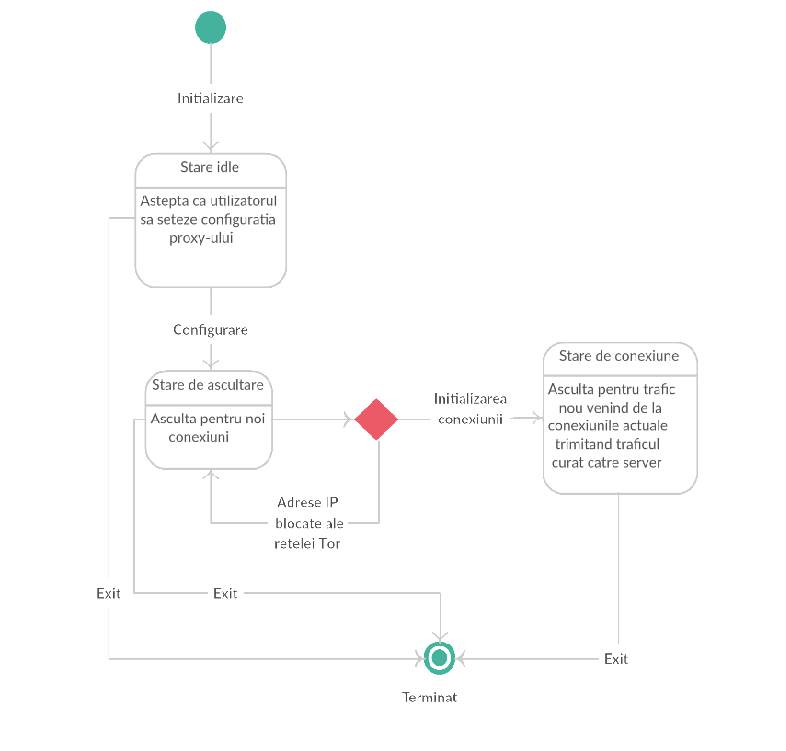
\includegraphics[width=0.8\textwidth]{state_diagram.png}
	\caption{Diagrama de stare a sistemului propus.}
	\label{fig:state}
\end{figure}
Figura ~\ref{fig:state} prezinta diagrama de stare a sistemului propus.

Dupa pornirea aplicatiei reprezentata prin initializare, utilizatorului i se pune la dispozitie interfata de utilizator in care sistemul asteapta sa fie configurat si portnit("Idle state"). Dupa configurarea aplicatiei in meniul "Configure",prin setarea specificatiilor serverului de reverse proxy, prin apasarea butonului "start", sistemul trece in urmatoarea stare "Listaning state". In aceasta stare sistemul accepta noi conexiuni de la diferiti clienti ce doresc sa acceseze server-ele protejate de acesta. Tot aici are loc si verificarea adreselor ip ale clientilor pentru protejarea importiva utilizatorilor Tor. Dupa stabilirea unei noi conexiuni, sistemul intra in starea "Connected state", in care acesta asculta pentru noi request-uri intre client si server si le trasmite mai departe catre destinatia dorita. Tot aici are loc si validarea request-urilor trimise de clienti catre server pentru prevenirea atacurilor SQL injection.
In aceasta stare utilizatorul poate sa urmareasca activitatea sistemului in meniul "Monitor" din interfata de utilizator, unde sunt logate toate evenimentele generate de sistem. Pentru oprirea aplicatiei, utilizatorul poate pur si simplu sa o inchida de la butonul din drapta sus, aceasta terminandu-si toata activitatea indiferent de starea in care se afla.

\begin{figure}[h]
	\centering
	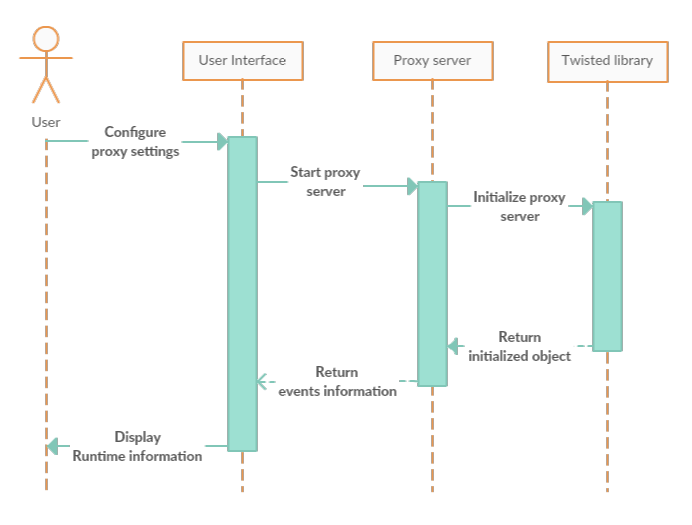
\includegraphics[width=0.9\textwidth]{sequence_diagram.png}
	\caption{Diagrama de secventa a sitemului propus.}
	\label{fig:sequence}
\end{figure}
Figura ~\ref{fig:sequence} prezinta diagrama de secventa a sitemului propus. \\
Dupa pornirea sistemului, utilizatorul configureaza setarile pentru server-ul de reverse proxy din interfata de utilizator(in meniul "Configure"). Dupa configurarea sistemului, prin apasarea butonului de start, este lansata in executie server-ul de reverse proxy cu caracteristicele specificate de utilizator. Scriptul de pornire a server-ului de reverse proxy face apel la fisierele bibliotecii Twisted, care vor returna catre acesta o instanta a serverului initializat. In interiorul server-ului de reverse proxy, aparitia de noi evenimente este semnalata catre interfata grafica. Aceste evenimente sunt puse la dispozitia utilizatorului pentru vizualizare.
\\
\section{Dependintele sistemului}

Pentru functionarea corecta a sistemului propus, acesta are nevoie de urmatoarele dependinte:
\begin{enumerate}
	\item Sistem de operare Windows cu Python2 instalat pe sistem.
	\item Conexiune stabila la internet pentru rularea script-urilor ce obtin adresele ip utilizate de Tor.
	\item Sistemul sa aiba acces direct la interfetele prin care clientii se pot conecta la server-ul protejat
	\item Sistemul sa aiba o conexiune directa la server-ul ce trebuie protejat.
\end{enumerate}
\section{Algoritmi si metode}

Pentru prevenirea atacurilor de SQL injection s-a folosit un algoritm de machine learning, support vector machine. Acest algoritm presupune antrenarea anterioara a unui model cu un set de date de referinta etichetate in prealabil corect de catre utilizator. Aceste date sunt folosite de algoritm pentru a raporta noi seturi de date, natura acestora fiind necunoscuta, incercand sa gaseasca similitudin intre cele noi si cele de referinta, determinandu-le astfel natura celor noi. Algoritmul de support vector machine rezulta intr-un model obtinut prin folosire a diversi algoritmi pentru antrenarea acestuia, folosit pentru a clasifica date.

Realizarea unui astfel de model sa realizat in urma executarii unui proces elaborat ce implica mai multi pasi:
\begin{itemize}
	\item  Primul pas reprezinta indentificarea datelor relevante in cea ce priveste problema tratata(prevenirea atacurilor SQL injection). In conformitate cu scopul clasificarii evenimentelor/datelor in doua categorii (tentativa de atac si request-uri clean) initial au fost  indentificate o serie de astfel de evenimente si categorizate in evenimente ce sigur apartin fiecarei dintre categoriile tinta. 
	\item Dupa  obtinerea datelor de antrenare, au fost indentificate toate trasaturile relevante din aceste date, trasaturi care sa fie cat se poate de specifice fiecarei categorii in parte. Aceste trasaturi au reprezentat cuvintele cheie a limbajului SQL dar si caractere specifice folosite frecvent de acesta.
	\item Dupa obtinerea trasaturilor specifice datelor de antrenare, sa realizat antrenarea modelului folosind un algoritm specific. In cazul proiectului propus s-a folsoit algoritmul gata implementat, furnizat de biblioteca open source LIBSVM \cite{libsvm}. Pentru obtinerea modelului datele de antrenare au fost procesate folosind un kernel gausian. Un kernel gausian reprezinta modul in care modelul proceseaza datele de antrenare astfel incat clasificarea noilor date sa fie realizata prin calcularea similaritatilor dintre acestea si cele de antrenare. In calcularea similaritatii dintre aceste doua tipuri de date, un parametru foare important este sigma. Acest parametru este ales pentru intrg setul de date, iar valoarea lui este diret proportionala cu gradul de similaritate pe care algoritmul il va asocia la doua evenimente/date diferite.
\end{itemize}

Pentru blocarea ip-urilor utilizate de reteua Tor s-a folosit un script scris in Python3. Programul interogheaza periodic(din 6 in 6 ore) informatiile oferite de \textit{Tor Network Status} \cite{tot_status}, salvand uptime-ul fiecarei adrese din ultimele 6 ore. Indentifiacrea adreselor malitioase se face prin insumarea timpului total din ultima luna de uptime, iar cele cu o valoare mai mare de 7 zile sunt considerate malitioase. Blocarea ip-urilor se realizeaza prin compoararea cu o astfel de lista generata lunar.

\section{Diagrama de desfasurare}
\begin{figure}[h]
	\centering
	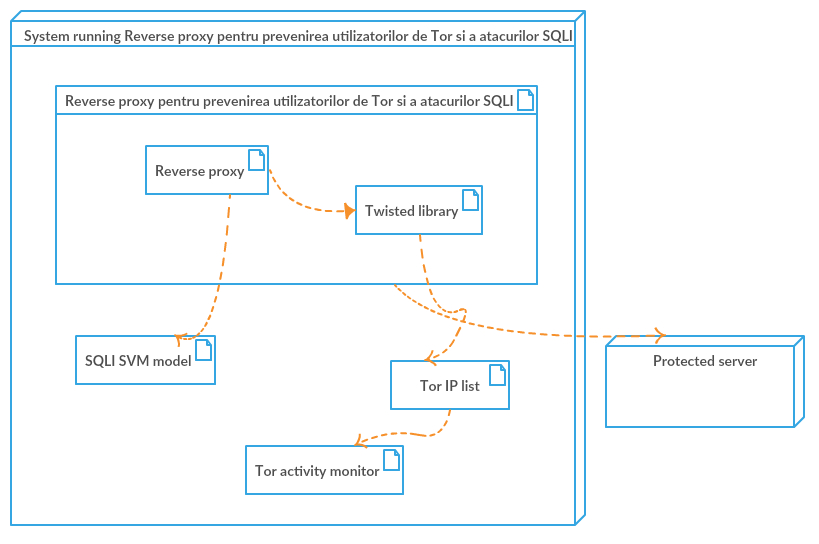
\includegraphics[width=0.8\textwidth]{deployment.png}
	\caption{Diagrama de desfasurare a sitemului propus.}
	\label{fig:deployment}
\end{figure}

Figura ~\ref{fig:deployment} prezinta diagrama de desfasurare a sitemului propus. \\
Pentru a putea rula sistemul \textit{\thesistitle} pe un sistem, acesta trebuie sa aiba acces direct la server-ul ce se doreste a fi protejat. Sistemuli trebuie sa ii fie frunizate modelul de SVM folosit pentru prevenirea atacurilor de SQL injection. De asemenea scriptul pentru monitorizarea activitatii retelei Tor si cel pentru generarea listei de adrese IP cu un uptime mai mare de 7 zile, trebuie sa se afle pe sistem, pentru ca acesta sa utilizeze date "up-to-date".

\section{Justificarea design-ului}
 

Totate deciziile de design au fost luate in vederea obtinerii unor functionalitati cat mai importante pentru utilizatorii tinta, dar si pentru a obtine o eficienta cat mai mare a sistemulu, atat din punct de vedere al corectitudinii cat si a timpului de executie.


Pentru o acuratete cat mai mare in prevenirea atacurilor de SQL injection s-a ales folosirea unui abordari bazate pe machine learning, intrucat detectiile statice prezinta o logica foarte complicata, pot omite multe cazuri esentiale si sunt limitate de capacitatea de observare a programatorului. 


Pentru indentificarea adreselor utilizate de reteaua Tor se putea aborda o implementare cu lista fixa, intrucat aceste liste prezinta un set mic de adrese ce raman neschimbate in timp, insa pentru o acuratete cat mai mare, s-a ales folosirea celor doua scripturi suplimentare ce vor obtine periodic toate adresele utilizate de retea perioada respectiva de timp.


De asemenea dezvoltarea modulara a sistemului asigura usurinta de adaugare de noi module sau functionalitati fara a necesita modificari majore sistemului actual.

%Acest capitol descrie design-ul proiectului și cuprinde, în general: 
%\begin{enumerate}
%  \item ilustrarea arhitecturii generale și detaliate a sistemului implementat, care să evidențieze modulele componente și relațiile dintre acestea
%  \item stările prin care trece sistemul în decursul funcționării sale (diagrame de stare)
%  \item modul de interacțiune dintre module și funcționalitatea acestora ilustrată prin diagrame de secvențe
%  \item descrierea algoritmilor/metodelor pe care se bazează funcționarea sistemului dezvoltat
%  \item descrierea organizării/structurii eventualelor baze de date folosite
%  \item justificarea alegerilor/deciziilor făcute și analiza critică a acestora (avantaje și dezavantaje), prin comparație cu alte alternative posibile
%\end{enumerate}
%
%Ca idee generală, design-ul trebuie să fie prezentat independent de o implementare anume, în general, și de cea a voastră, în particular. De asemenea, descrierea design-ului trebuie să conțină toate elementele și detaliile necesare, astfel încât altcineva decât voi să poate realiza o implementare a lui, fără a fi nevoit să ia decizii arhitecturale sau organizare (adică, de design) și să vă contacteze pentru a-și lămuri anumite aspecte neclare.
%
%Capitolul trebuie organizat pe secțiuni și subsecțiuni astfel descrierea să urmeze un cors logic și ușor de urmărit. 
%
%Ponderea acestui capitol relativ la întreaga lucrare este de 25-35\%.
%
%
%\section{Examples: lists, figures, tables, equations}
%
%Așa arată o listă de elemente nenumerotate:
%\begin{itemize}
%  \item element 1
%  \item element 2
%  \item \dots
%\end{itemize}
%
%
%Așa arată o listă de elemente numerotare:
%\begin{itemize}
%  \item element 1
%  \item element 2
%  \item \dots
%\end{itemize}
%
%
%Așa arată o listă în text: 
%\begin{inparaenum}[(\itshape 1 \upshape)]
%  \item element 1, 
%  \item element 2, 
%  \item \dots
%\end{inparaenum}
%
%\textbf{Atenție}: orice tabel, figura sau ecuație (formulă) trebuie referite \textit{explicit} în text explicit (de genul: în Figura X este ulustrat \dots, în Tabelul Y se poate vedea \dots), pentru că Latex le poate plasa chiar și pe altă pagină decât acolo unde vrem noi să ne referim la ele. Vedeți exemple de mai jos!
%
%Tabelul~\ref{table:example} ilustrează un exemplu de tabel. Un editor on-line de tabele poate fi găsit la \url{http://www.tablesgenerator.com/}. 
%
%\begin{table}[t]
%\centering                          % tabel centrat 
%\begin{tabular}{|c|c|c|c|}          % 4 coloane centrate 
%\hline\hline                        % linie orizontala dubla
%Case & Method\#1 & Method\#2 & Method\#3 \\ [0.5ex]   % inserare tabel
%%heading
%\hline                              % linie orizontal simpla
%1 & 50 & 837 & 970 \\               % corpul tabelului 
%2 & 47 & 877 & 230 \\
%3 & 31 & 25 & 415 \\[1ex]           % [1ex] adds vertical space
%\hline                              
%\end{tabular}
%\caption{Nonlinear Model Results}   % titlul tabelului
%\label{table:example}                % \label{table:nonlin} introduce eticheta folosita pentru referirea tabelului in text; referirea in text se va face cu \ref{table:nonlin}
%\end{table}
%
%În Figura~\ref{fig:exemplu} 
%
%\begin{figure}
%    \centering
%    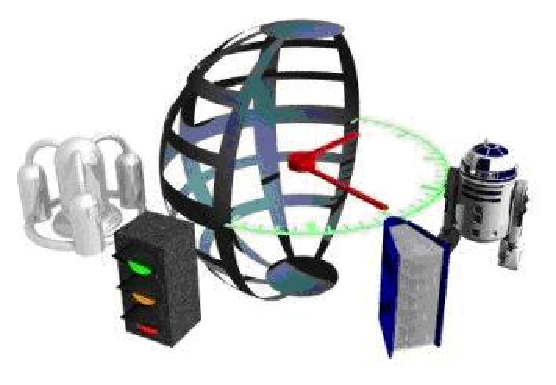
\includegraphics[width=0.5\textwidth]{image}
%    \caption{Numele figurii}
%    \label{fig:exemplu}
%\end{figure}
%
%
%Formula~(\ref{eq:example}) arată modul de calcul al lui $\Delta$:
%\begin{equation} \label{eq:example}
%    \Delta =\sum_{i=1}^N w_i (x_i - \bar{x})^2 .
%\end{equation}
%
%
%Algoritmul~\ref{alg:example} este un exemplu de descriere pseudo-cod a unui algoritm, preluat de la \href{http://en.wikibooks.org/wiki/LaTeX/Algorithms#Typesetting_using_the_algorithm2e_package}{http://en.wikibooks.org/wiki/LaTeX}. El utilizează pachetul \textit{algorithm2e}. Alternativ, puteți utiliza pachetele \textit{algorithmic} sau \textit{program}. 
%
%\begin{algorithm}
% \KwData{this text}
% \KwResult{how to write algorithm with \LaTeX2e }
% initialization\;
% \While{not at end of this document}{
%  read current\;
%  \eIf{understand}{
%   go to next section\;
%   current section becomes this one\;
%   }{
%   go back to the beginning of current section\;
%  }
% }
% \caption{How to write algorithms}
% \label{alg:example}
%\end{algorithm}
